% -*- coding: utf-8 -*-

\section{Algorithms}
\label{algorithms}

\subsection{Introduction}
In this section I will go into high-level detail about the principal problems that are to be solved in this project, as well as the algorithms that I have used to solve them. With each algorithm I will include an explanation of their use, an analysis of the algorithms run-time. At the end of this section I will also discuss the general efficiency of the RSS and the how to minimize the volume.
The 3 algorithms I will go into detail in this section is the overlap algorithm, the creation of RSS from a set of points, and the creation of a new RSS from 2 other RSS'.

\subsection{Overlap}
\label{overlap}
In order to be able to use the Rectangular Swept Sphere (RSS) in ProGAL framework, I must implement a method to detect whether 2 RSS' are overlapping, so that it can be decided whether a confirmation of the protein should go ahead or not. In the following I will describe the methods I have used to check whether or not two RSS' are overlapping.

\subsubsection{Approach}
In the algorithm I have chosen to implement, I will prefer to report a possible overlap where there might not be one, instead of failing to report a possible overlap. In theory this can happen with the current implementation of RSS overlap algorithm, but in practice false positives are not very likely, though see section \ref{realWorldData}.

The algorithm is split into 2 phases: The minimum distance test and the axis-separation test. The first test finds the minimum distance between the rectangles of the RSS'. If the found distance is less than the combined radius, then we can report an overlap. However, since the current implementation of the Minimum distance algorithm only works when the 2 closest  points both lie on an edge, there is a need for the axis-separation test, which checks whether there exists an axis separating the 2 RSS' (in which case they cannot overlap). The axis-separation test is likely to take longer than the Minimum distance check, but it will always correctly identify whether the 2 RSS overlaps or not.

\subsubsection{Minimum distance}

\begin{figure}
\centering
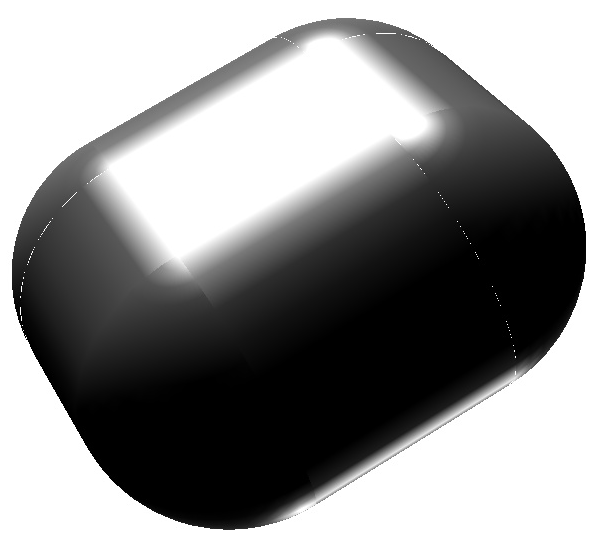
\includegraphics[width=0.5\textwidth]{figures/normalInter}
\caption{\label{normal-inter}An example of 2 RSS overlapping}
\end{figure}

In the following let minDist(rec(A), rec(B)) be the minimum distance between the rectangles of RSS A and B, radius(A) is the radius of A.\\

One approach to check if 2 RSS', A and B, overlap, is to check the minimum distance between their rectangles. It is clear that if minDist(rec(A), rec(B)) $<=$ Radius(A) + radius(B)  (see figure \ref{normal-inter} for an illustration) then A and B must overlap. This is the approach found in \cite{Larsen99fastproximity} and \cite{larsen00fast}, which I have tried to implement in this project.

The problem then becomes one of finding the 2 closest points between rec(A) and rec(B), and calculating their distance.

According to section 4.2.1 of \cite{Larsen99fastproximity} the possible configurations of the closest points are, 
\begin{enumerate}
\item Both of the points lie on an edge. This is the situation illustrated in figure \ref{normal-inter}. This is the only case where \cite{Larsen99fastproximity} uses the minimum distance algorithm.
\item One of the points lie in the interior of one of the rectangles (where the other point lies is irrelevant). This is the case is illustrated in figure \ref{parallel}. To handle this case, both I use the Axis-separation algorithm. 
\end{enumerate}

\subsection{Minimum distance}
\label{minimumDistance}
I will only deal with minimum distance in the case where the 2 closest points both lies on the edges of the RSS'.

It is clear that if the 2 closest points lie on the edges, then the naively approach would be to find the smallest distance from all edges from RSS A to all edges on RSS B, and then returning the smallest of these. This would however require 16 distance calculations, some of which clearly unnecessary - for instance doing any distance calculations for edge e in figure \ref{vor-cheap}, since it is the edge furthest away from the other RSS. 

Thus we are only in interested in doing distance calculations between the edges that are closest together. The approach in my implementation is the one described in \cite{larsen00fast} and \cite{Larsen99fastproximity}, where the authors exploit the properties of Voronoi diagrams. Given a set G of geometric structures (points, line-segments, etc.) in an n-dimensional space, a Voronoi diagram can be used to find the set of points are closets to any member of G. A formal definition of Voronoi diagrams can be found in \cite{compgeom:2008} Chapter 7. In this case the Voronoi diagrams should be used on line-segments from one of the RSS', and the resulting diagram would allow us to identify which pair of edges are worth checking.

The interested reader might want to read \cite{larsen00fast} section 4.2 and \cite{Larsen99fastproximity} section 4.3.1 (especially Lemma 1) - for a more in-depth treatment of Voronoi diagrams in relation to this.

\begin{figure}
\centering
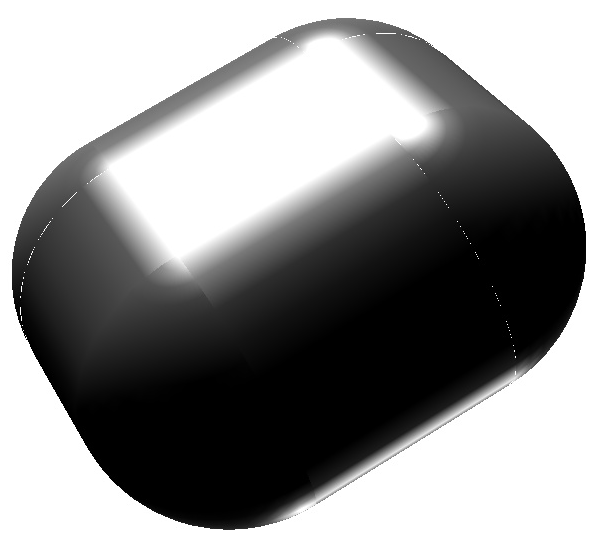
\includegraphics[width=\textwidth]{figures/vorCheap}
\caption{\label{vor-cheap}An illustration of the cheap Voronoi diagram method (shown in 2d for simplicity). The letters indicate with edges are closest to that area. Areas which multiple letters will be checked by multiple edges. For instance, the edges of RSS2 that either lie completely, or partially in area 3 will be checked by both RSS1's edge a and d. The edges of RSS2 that lies entirely within area 5 will only be checked by RSS1's edge d.}
\end{figure}

Fortunately I do not need to calculate the Voronoi diagram in order to detect which Voronoi cell an edge/line-segments lies in. Let E be the edge on the rectangle whose closest edges we wish to find, \textbf{n} be an arbitrary vector perpendicular to E, pointing away from the interior of the rectangle, then the face defined by -\textbf{n} and a point on E will define the half-plane D. All edges/line-segments that lies, wholly or partly, within D are candidates for the closest edge, as described in \cite{larsen00fast}. Using this approach, instead of explicitly calculating the Voronoi diagram, has the disadvantage that an edge might lie in multiple half-planes. However, even in the worst case we would have to perform 8 Minimum distance calculations, which still is an improvement compared to doing 16 Minimum distance calculations. See figure \ref{vor-cheap} for an illustration of approach used both in this project and \cite{larsen00fast} and \cite{Larsen99fastproximity}.

Now that we have reduced the number of Minimum distance calculations, the problem becomes one of finding the minimum distance between 2 line-segments in 3 dimensions, and then returning the smallest of these values. If no possible candidates are found, then infinity is returned.

The algorithm I uses to find the minimum distance between the line-segments is as follows:\\
\begin{algorithm}[H]
  \caption{Mindistane line-segments}
  \label{mindist-lineseg}
  \SetKwData{return}{return}
  \SetKwInOut{Input}{input} \SetKwInOut{Output}{output}
  \dontprintsemicolon
  \Input{lineSeg1 and lineSeg2, the 2 line-segments we want to compare. p1 and p2, two points on the line-segments}
  \Output{The distance between the line-segments}
   pointVector $\gets$ makeVektor(p1, p2) \;
   a $\gets$ dotProduct(lineSeg1, lineSeg1) \;
   b $\gets$ dotProduct(lineSeg1, lineSeg2) \;
   c $\gets$ dotProduct(lineSeg2, lineSeg2) \;
   d $\gets$ dotProduct(lineSeg1, pointVector) \;
   e $\gets$ dotProduct(lineSeg2, pointVector) \;
   dominator $\gets$ a * c + b * b \;
   \eIf{dominator == 0.0}{
     line1Mul $\gets$ (b * e - c * d) / dominator \;
     line2Mul $\gets$ (a * e - b * d) / dominator \;
     line1Clone $\gets$ mult(lineSeg1, edge1Mul); \;
     line2Clone $\gets$ mult(lineSeg2, edge2Mul); \;
     line1Clone $\gets$ add(line1Clone, pointVector) \;
     line1Clone $\gets$ subtract(line1Clone, line2Clone) \;
     \return length(line1Clone) \;
   }{
     \return length(pointVector) \;
   }  
\end{algorithm}

\subsection{Axis separation test}
\label{sepAxis}

In order to take care of the cases where 2 rectangles either overlap or where the closest point lies inside the interior of the rectangles, I have to do an Axis-separation check. The gist of the Axis-separation test is ``that two disjoint convex polytopes in 3-space can always be separated by a plane which is parallel to a face of either polytope, or parallel to an edge from each polytope'' (\cite{237244}, section 5, page. 8).

The Axis-separation test described in \cite{237244} was designed to work on Oriented Bounding Boxes (OBB's). For the RSS this means that an OBB containing the RSS must be constructed at the creation of a RSS (see also section \ref{multiple-points}). 

The Axis separation test works by generating a unit plane, and by projecting the length of the OBB onto this plane. If, at least one of the projections are disjoint, then the 2 OBB's (and hence the 2 RSS'), must be disjoint.

In all 15 planes have to be tested for axis separation. The first 6 planes comes from the 3 faces for each of the 2 OBB; and the last 9 planes are the 9 pairwise combination of edges from the 2 OBBs. 

\subsubsection{Order of Minimum distance and Axis separating test}
\label{minAxisOrder}
An important question is whether running the minimum distance test, followed by the axis-separation is optimal, or if it might be better just to run the axis separation test.

It is important to understand the purpose of the methods, and the cases that terminates the algorithms, which cases makes them terminate earliest, and well as the cases that makes them do the most work.

\begin{figure}
\centering
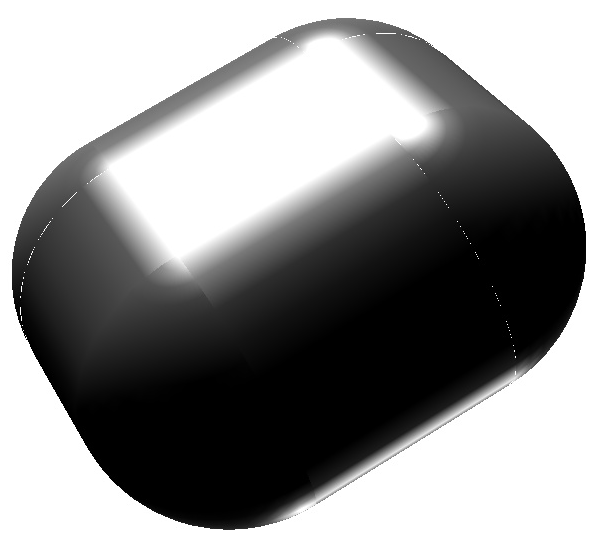
\includegraphics[width=\textwidth]{figures/sepAxis}
\caption{\label{parallel} A RSS lies above, and inside another RSS.}
\end{figure}

\subsubsection{Minimum distance}
\begin{description}
\item[Purpose:] The minimum distance algorithm tries to find the minimum distance between 2 RSS'.
\item[Terminating condition:]The terminating condition of the minimum-distance algorithm is when it has either checked all edges for minimum distance, or when it finds a minimum distance that is smaller than the combined radius of the RSS'. If the algorithm returns true, then we know that the 2 RSS' overlap, but if it returns false, then we do not know whether the 2 RSS' overlap or not.
\item[Best case:] The first edge is closer than the combined radius of both RSS' - the test returns true and terminates.
\item[Worst case:] All the edges are tested, but we found distance is greater than the combined radius. Nothing concrete can be gained from this case.
\item[Does not handle:] This algorithm cannot handle cases where one of the RSS lies ``above'' or ``below'' the other (in the plane generated by the second's RSS' rectangle). See figure \ref{parallel} for an illustration of the case.
\end{description}

\subsubsection{Axis-separation test}
\begin{description}
\item[Purpose:] The axis separation algorithm tries to find an axis that separates the 2 RSS'. 
\item[Terminating condition:] The axis-separation test terminates either when it finds an axis which separates the 2 OBBs' that contain the RSS, or after having run all 15 axis-tests.
\item[Best case:] The first axis test shows that the 2 RSS' are disjoint, and the algorithm terminates. 
\item[Worst case:] The 2 RSS' are not disjoint, and so all 15 axis-tests have to be made.
\item[Does not handle:] Axis-separation test handles all cases.
\end{description}

It is thus clear that the worst case where RSS A overlaps with RSS B in B's interior - since this case is not handled by the minimum distance test, and the Axis-separation test will have to do all 15 tests. 

If we think that it is likely that a RSS will lie in the interior or another (either overlapping, or lying above or below the RSS' rectangle) or that RSS' will only overlap in rare cases, then it will be a better only run the Axis-separation test. If, on the other hand, we believe RSS' are unlikely to lie above/below each others rectangle, and will often overlap, then the minimum distance algorithm, followed by the Axis-separation test will be a better choice.

Since in the context of folding proteins are interested in being told that a confirmation creates an overlap as soon as possible (so that the next possible conformation can be tested\footnote{In a BVH, and thus in practice, we furthermore have the case that a detected overlap will lead to further tests - making it very important that overlap test can be done quickly}), I think that first running the Minimum distance algorithm, and then the Axis-separation test would improve the run-time in most instances, instead of only running the Axis-separation test.

\subsubsection{Asymptotic run time}
Both the minimum distance and the axis-separation algorithm runs in $O(1)$.

\subsection{Creating RSS from multiple points}
\label{multiple-points}
In order for the RSS to be a useful BV, it is clear that I have to find an algorithm that given a set of points can construct a RSS that contains them all. The primary metric should be the volume.

In the implemented algorithm I first create a OBB, which I use to find the length, width, radius and center point of the RSS. In order to identify the vectors for the RSS, create a set of eigen vectors from point set (a optimization would be to just use the vectors from the created OBB). I then sort the eigen vectors according to their eigenvalues (in a descending order), in order to easily find the 1st and 2nd principal component. With the help of these I can create the RSS' rectangle, and from that the RSS itself. In order to be able to perform the Axis separation test correctly and efficiently, I add the radius to the length and width of the OBB, so that the OBB contains the entirely, and then add let the RSS contain the OBB. 

\begin{algorithm}[H]
  \caption{CreateRSSContainingPoints}
  \label{create-algo}
  \SetKwData{covar}{CovarianceMatrix}
  \SetKwData{eigen}{EigenVectors}
  \SetKwData{threedeeRec}{3dRec}
  \SetKwData{return}{return}
  \SetKwData{p}{p}
  \SetKwData{obox}{obbBox}
  \SetKwData{rss}{rss}
  \SetKwInOut{Input}{input} \SetKwInOut{Output}{output}
  \dontprintsemicolon
  \Input{A set P of n points in 3 dimensions}
  \Output{A RSS that contains all points in P}
  \covar $\gets$ makeCovarainceMatrix(P)\;
  \eigen $\gets$ getEigen(\covar) \;
  \eigen $\gets$ sort(\eigen) \;
  \obox $\gets$ makeOBB(points) \;
  length = \obox.length\;
  width = \obox.width\;
  radius = \obox.height \;
  centerPoint $\gets$ \obox.getCenter() \;
  \threedeeRec $\gets$ 3dRec(centerPoint, \eigen[1].scaledTo(width), \eigen[0].scaledTo(length)) \;
  \rss $\gets$ RSS(\threedeeRec, radius) \;
  \obox.length += radius \;
  \obox.width += radius \;
  \rss.\obox = \obox \;
  \return rss
\end{algorithm}

\subsubsection{Asymptotic Runtime}
The subroutine that finds the covariance matrix for algorithm \ref{create-algo} runs in $O(n)$. The subroutine that creates the OBB runs in $O(n)$, and everything else runs in constant time. Thus the algorithm must have an asymptotic run-time of $O(n)$.

\subsection{Algorithm to create a RSS containing 2 RSS'}
In order to combine  2 RSS', rss1 and rss2, I take the corner points of the 2 RSS', and create a new RSS rss3 from the combined point-set. I then take the maximum of radii from rss1 rss2, and add it to the radius of rss3 and the OBB that is associated with rss3. The extra radius has to be added, since otherwise some of the points on rss1 and rss2 contain will not be contained in rss3. 

\begin{algorithm}[H]
  \caption{CombinedRSS}
  \label{combine-algo}
  \SetKwData{points}{pointsSet}
  \SetKwData{crss}{rss3}
  \SetKwData{return}{return}
  \SetKwInOut{Input}{input} \SetKwInOut{Output}{output}
  \dontprintsemicolon
  \Input{2 RSS' rss1 and rss2}
  \Output{A RSS that contains both RSS'}
  Initialize \points \;
  Add cornerPoints(rss1) and cornerPoints(rss2) to \points \;
  \crss $\gets$ CreateRSSContainingPoints(\points) \;
  maxRadius $\gets$ max(radius(rss1), radius(rss2)) \;
  add maxRadius to the length and width of the box contained in \crss\;
  \crss.radius $\gets$ \crss.radius + maxRadius \;
  \return \crss \;
\end{algorithm}

\subsubsection{Asymptotic Runtime}
It is clear that algorithm \ref{combine-algo} must run in $O(1)$, since the point set we used to create the rss will always contain 8 points, and all other operations takes constant time. 

\subsection{Efficiency}
I will in the following assume that all RSS are created in order to contain a point set. Let a normal RSS be an RSS as they are currently created where all the points that defines the RSS are contained in an OBB inside the RSS (i.e. no points lie in the half-cylinder part on the edges of the RSS) - see \ref{rim} for an illustration. 

From section \ref{rss} it is clear that a naively created RSS will just create a OBB around the points, together with 2 cylinders around the edges. From this it is clear that if RSS are ever to be more efficient than a OBB, then either the naive method at generating a RSS has to be replaced, and the properties that separates the RSS from the OBB must be exploited. 

For talks on optimizing the volume see section \ref{optimized-volume}. The only real property that all RSS' apart from OBB's, is the radius. This is what we are trying to exploit in the minimum distance check. It is is therefore clear that in order to optimize the overlap algorithm for RSS', the effort should be focused on the Minimum distance check. As detailed in the section \ref{results}, it is therefore clear the currently implemented minimum distance check does not currently make the RSS BV faster than the OBB for overlap detection. I am however confident that there must exist a faster algorithm to check the distance between 2 line-segments. 
Furthermore, as I mentioned in section \ref{lit}, I have misunderstood some of the finer points of both \cite{Larsen99fastproximity} and \cite{larsen00fast}, which was to be an expansion of the minimum distance check, which would avoid axis-separation entirely. 

\subsection{Optimized volume}
\label{optimized-volume}
\begin{figure}
\centering
\includegraphics[width=0.5\textwidth]{figures/rim}
\caption{\label{rim} An illustration (seen from above) of an RSS created by the current implementation. It is clear that the radius around the rectangle (in the x and y-coordinate) is superfluous, and that a much tighter fit could be archived}
\end{figure}

In the current implementation of algorithm \ref{combine-algo}, the created RSS is essentially an OBB with the radius tacked on on the sides. This is clearly not optimal, as illustrated in figure \ref{rim}. It is clear that we cannot reduce the radius, since this would mean we would miss some of the points that lies above and below the rectangle. Thus we can only reduce the volume by reducing the length and width of the rectangle. This however, is not a trivial task. For instance, just reducing the length and the width with the radius is not sure to resolve in a legal RSS, as some of the points might lie in the corners of the OBB, and will thus in the new RSS lie just outside the rounded corners. This problem is also highlighted in \cite{Larsen99fastproximity} section 4.1, where they, deal with it, in practice, increasing both the length and the width of the rectangle by the same amount, until all points are covered.

A possible solution, which has not been implemented in this project, could be to start with a minimal rectangle, i.e. a rectangle where the radius has been subtracted from both the width and the length. Then, for each point in the point set that defines the RSS, we compare the minimum distance $\delta$ from the current rectangle and the radius r. If $\delta <=$ r, then the point is inside the current RSS, and nothing has to be done, if however $\delta >$ r, then both the width and the length is increased by the $\delta -$ r, so that the point that before lay outside the RSS now lies inside of it\footnote{Since we only increase the width and length, we can be sure that the points that have been checked before will still lie inside the RSS}.
 
\subsection{Conclusion}
I have in this section presented the main problem that my algorithms are trying to solve - to find out whether 2 RSS' overlap, how to create a RSS from a point set, and how to create a new RSS that will contain all the points of 2 other RSS'. I have presented all the algorithms on both high- and low-level, which possibilities exist to archive a RSS whose overlap has a better run time than the OBB, and at the end a discussion on how to improve upon the fit of the RSS.
